\documentclass[fleqn]{beamer}

\usepackage[british]{babel}
\usepackage{graphicx,ru,url}
\usepackage{amsmath,amsfonts}
% Use Times for math font and text font.
\RequirePackage[T1]{fontenc}
%\RequirePackage{txfonts}
% bold math must be loaded after Times font
\usepackage{bm}
\usepackage{booktabs} % nice rules (thick lines) for tables
\usepackage{microtype} % improves typography for PDF
\usepackage{xcolor}
\usepackage{tikz}
\usepackage{verbatim}
\usetikzlibrary{arrows,shapes, decorations}
\usepackage{hyperref}

\graphicspath{{figures/}} % Specifies the directory where pictures are stored

% \usefonttheme{serif}

\providecommand{\e}[1]{\ensuremath{\times 10^{#1}}}

% The title of the presentation:
%  - first a short version which is visible at the bottom of each slide;
%  - second the full title shown on the title slide;
\title[KLT Basis for Energy Expansion]{
    Applications of the Karhunen-Lo\`{e}ve Transform to the C5G7 benchmark in
    the Response Matrix Method}

% Optional: a subtitle to be displayed on the title slide
%\subtitle{Show where you're from}

% The author(s) of the presentation:
%  - again first a short version to be displayed at the bottom;
%  - next the full list of authors, which may include contact information;
\author[Richard Reed]{
    Richard Reed \\
    Prof. Jeremy Roberts}

% The institute:
%  - to start the name of the university as displayed on the top of each slide
%    this can be adjusted such that you can also create a Dutch version
%  - next the institute information as displayed on the title slide
\institute[Kansas State University]{
    Mechanical and Nuclear Engineering \\
    Kansas State University}

% Add a date and possibly the name of the event to the slides
%  - again first a short version to be shown at the bottom of each slide
%  - second the full date and event name for the title slide
\date[ANS Winter Meeting 2015]{
    ANS Winter Meeting \\
    November 2015}

\begin{document}
    %\renewcommand*{\inserttotalframenumber}{\pageref{lastframe}}
    \newcommand{\beginbackup}{
        \newcounter{framenumbervorappendix}
        \setcounter{framenumbervorappendix}{\value{framenumber}}
    }
    \newcommand{\backupend}{
        \addtocounter{framenumbervorappendix}{-\value{framenumber}}
        \addtocounter{framenumber}{\value{framenumbervorappendix}}
    }

    \begin{frame}
        \titlepage
    \end{frame}

    \begin{frame}
        \frametitle{Outline}
        \begin{block}{Presentation Outline}
            \begin{itemize}
                \item Introduction and Background
                \begin{itemize}
                    \item Response Matrix Method
                    \item Energy Expansion
                    \item Basis Sets
                \end{itemize}
                \item C5G7 Test Problem and Models
                \item Results
                \item Conclusions
            \end{itemize}
        \end{block}
    \end{frame}

    \section{Introduction and Background}

    \begin{frame}
        \frametitle{Response Matrix Method}
        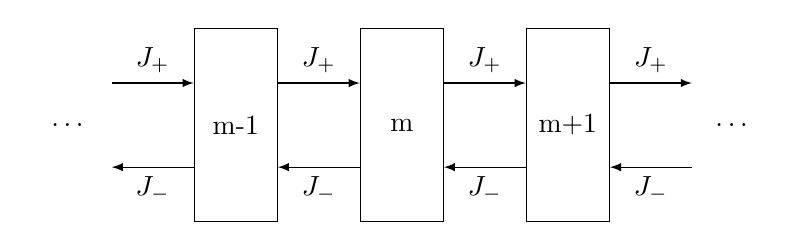
\begin{tikzpicture}[>=latex]
            %[set style={{help lines}+=[dashed]}, scale=0.85,
            %every node/.style={scale=1}]
            \tikzstyle{state} = [draw, fill=white, rectangle,
            minimum height=7em, minimum width=3em, node distance=6em]
            \tikzstyle{state2} = [draw=white, fill=white, rectangle,
            minimum height=7em, minimum width=3em, node distance=6em]
            \tikzstyle{stateEdgePortion} = [black];
            \tikzstyle{stateEdge} = [stateEdgePortion,->];
            \tikzstyle{edgeLabel} = [above, pos=0.5, text centered];
            \tikzstyle{edgeLabel2} = [below, pos=0.5, text centered];
            \node[state] (nodeM) {m-1};
            \node[state, right of=nodeM] (nodeN) {m};
            \node[state, right of=nodeN] (nodeO) {m+1};
            \node[state2, left of=nodeM] (nodeL) {\ldots};
            \node[state2, right of=nodeO] (nodeP) {\ldots};

            \draw (nodeM.45)
            edge[stateEdge] node[edgeLabel]{$J_+$}
            (nodeN.135);
            \draw (nodeN.45)
            edge[stateEdge] node[edgeLabel]{$J_+$}
            (nodeO.135);
            \draw (nodeO.45)
            edge[stateEdge] node[edgeLabel]{$J_+$}
            (nodeP.135);
            \draw (nodeL.45)
            edge[stateEdge] node[edgeLabel]{$J_+$}
            (nodeM.135);

            \draw (nodeN.225)
            edge[stateEdge] node[edgeLabel2]{$J_-$}
            (nodeM.315);
            \draw (nodeP.225)
            edge[stateEdge] node[edgeLabel2]{$J_-$}
            (nodeO.315);
            \draw (nodeO.225)
            edge[stateEdge] node[edgeLabel2]{$J_-$}
            (nodeN.315);
            \draw (nodeM.225)
            edge[stateEdge] node[edgeLabel2]{$J_-$}
            (nodeL.315);
        \end{tikzpicture}
        \begin{block}{Overview}
            \begin{itemize}
                \item Breaks global domain into independent nodes
                \item Nodes are linked by boundary conditions.
                \item Boundary conditions based on truncated, orthogonal
                basis expansions
                \item Sweep across nodes for global solution
            \end{itemize}
        \end{block}
    \end{frame}

    \begin{frame}
        \frametitle{The Multigroup Solution and the Kronecker-$\delta$}
        \begin{equation*}
            P_{\delta}^h(g) = \delta_{h, g-1} =
            \begin{cases}
                1, & \text{if }  h = g-1 \, , \\
                0, & \text{if }  h \neq g-1 \, .
            \end{cases}
            ,\, g=1,\, 2, \, \ldots,\, G \, ,
        \end{equation*}
        \begin{columns}[T]
            \begin{column}{0.5\textwidth}
                For the 4-group case, the Kronecker-$\delta$ vectors are:
                \begin{equation*}
                    \begin{align}
                        &[1,0,0,0] \\
                        &[0,1,0,0] \\
                        &[0,0,1,0] \\
                        &[0,0,0,1]
                    \end{align}
                \end{equation*}
            \end{column}
            \begin{column}{0.5\textwidth}
                \begin{block}{Overview of Kronecker-$\delta$}
                    \begin{itemize}
                        \item Prohibitively expensive with large G
                        \item Cannot truncate the basis set
                        \item Perfect convergence at full order
                    \end{itemize}
                \end{block}
            \end{column}
        \end{columns}
    \end{frame}

    \begin{frame}
        \frametitle{Modified Discrete Legendre Polynomials}
        \begin{columns}[T]
            \begin{column}{0.4\textwidth}
                \begin{block}{Creating mDLPs}
                    \begin{itemize}
                        \item Impose spatially averaged flux profile
                        \item Resulting polynomials are orthogonalized
                        \item Improves DLP by incorporating relevant phase
                        space
                        information
                    \end{itemize}
                \end{block}
            \end{column}
            \begin{column}{0.6\textwidth}
                \centering
                \only<1>{
                    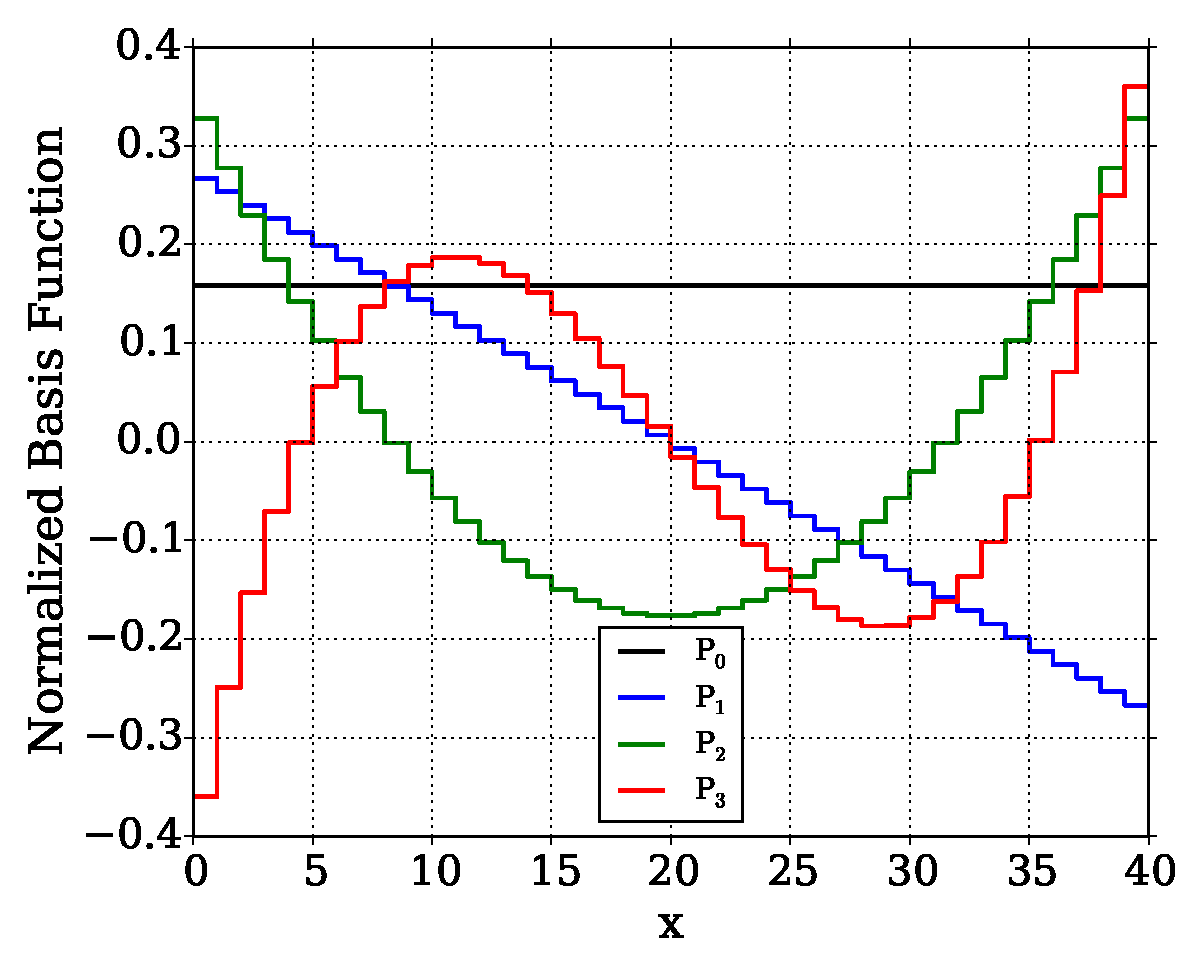
\includegraphics[trim=.1cm .25cm .1cm .4cm, clip=true,
                    totalheight=0.65\textheight]{Figures/DLP_basis}

                    DLP}

                \only<2>{
                    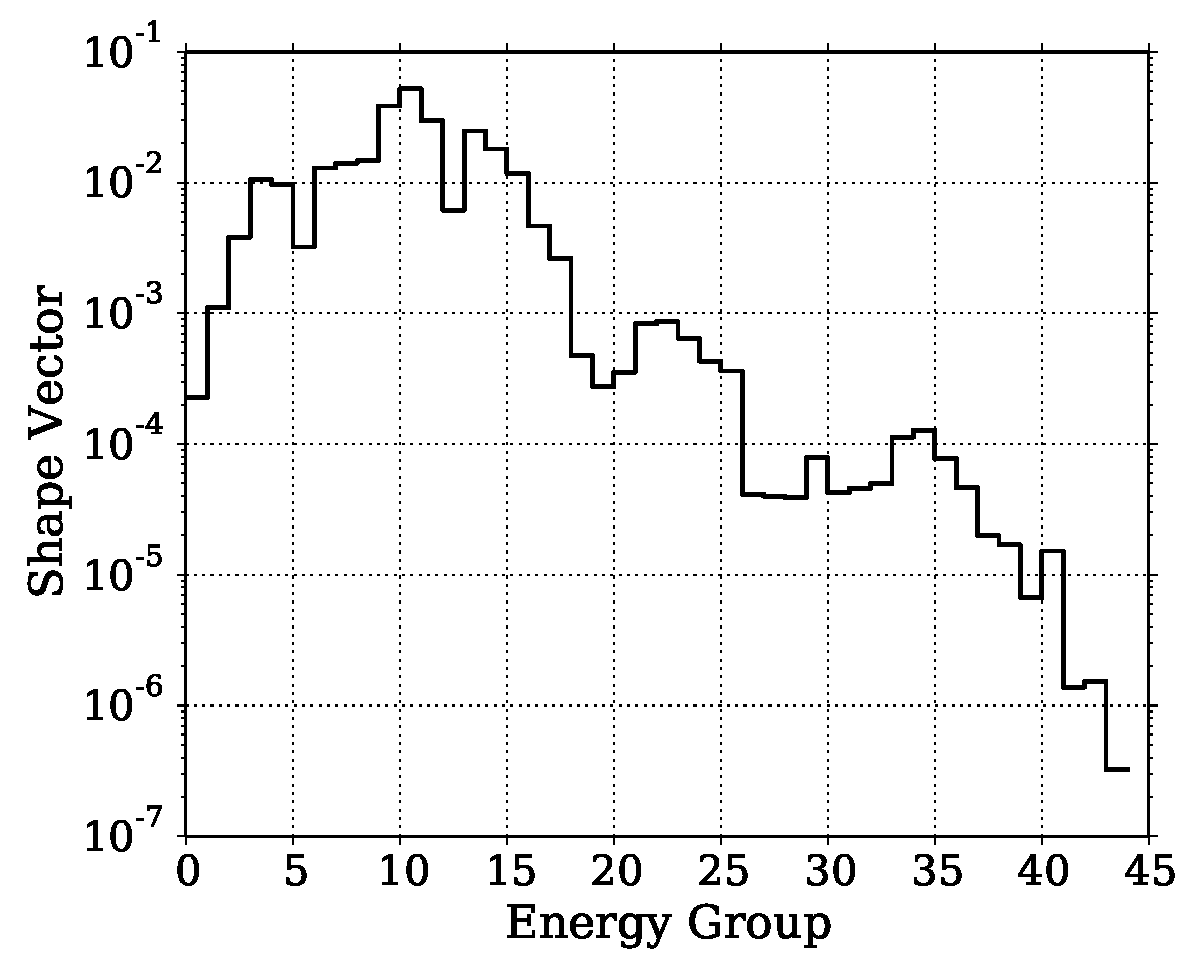
\includegraphics[trim=.1cm .25cm .1cm .4cm, clip=true,
                    totalheight=0.65\textheight]{Figures/shape}

                    Shape Vector}
                \only<3>{
                    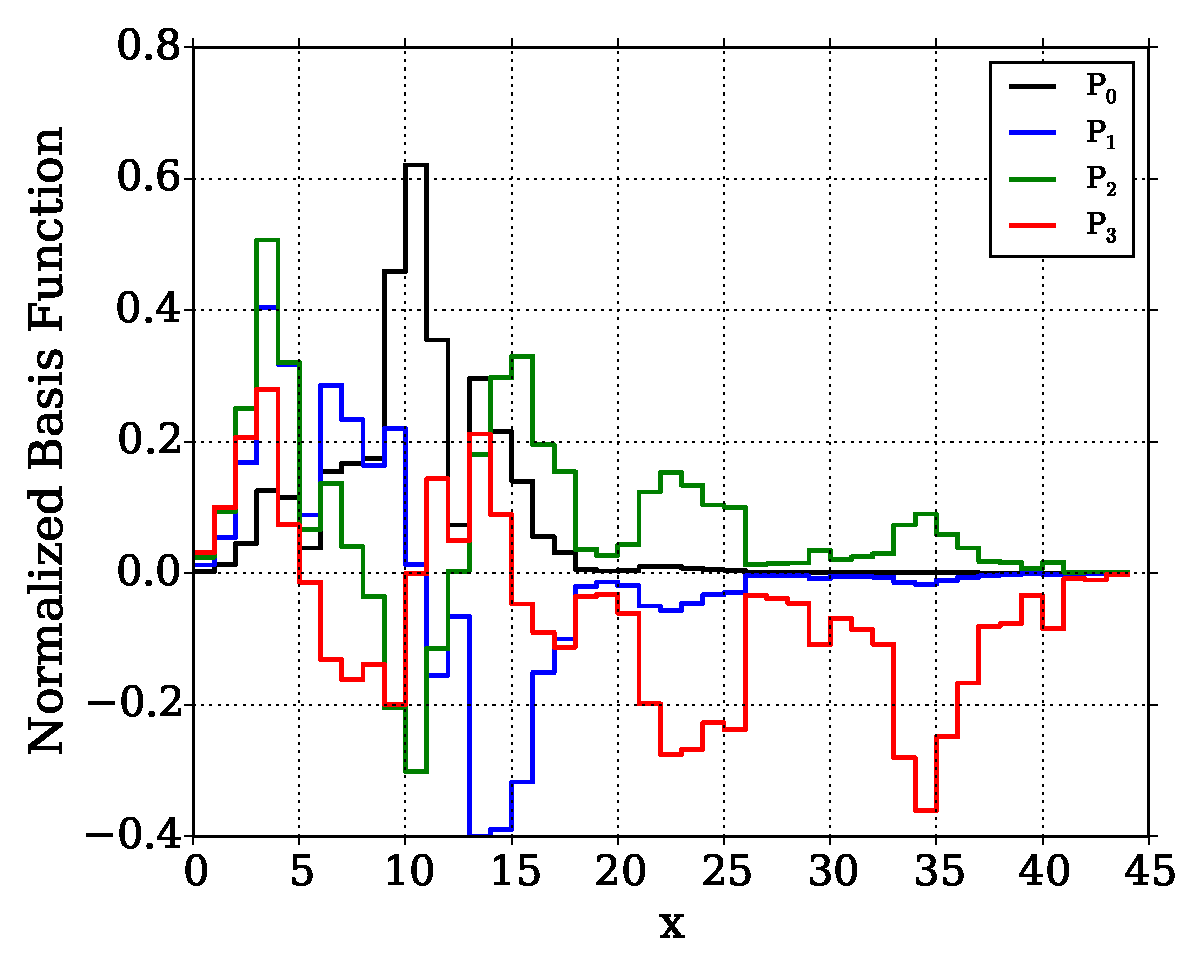
\includegraphics[trim=.1cm .25cm .1cm .4cm, clip=true,
                    totalheight=0.65\textheight]{Figures/mDLP1_L_basis}

                    mDLP}
            \end{column}
        \end{columns}
    \end{frame}

    \begin{frame}
        \frametitle{Karhunen Lo\'{e}ve Transform}
        \begin{block}{}
            Form matrix $\mathbf{D}$ from snapshots of $\phi$ or other term of
            interest.
        \end{block}
        \begin{columns}[c]
            \begin{column}{0.5\textwidth}
                \begin{equation*}
                    \mathbf{D} = \begin{bmatrix}
                        \phi_{1,1} & \phi_{1,2} & \cdots & \phi_{1,s} \\
                        \phi_{2,1} & \phi_{2,2} & \cdots & \phi_{2,s} \\
                        \vdots & \vdots & \ddots \\
                        \phi_{g,1} & \phi_{g,2} & & \phi_{g,s}
                    \end{bmatrix}
                \end{equation*}
            \end{column}
            \begin{column}{0.5\textwidth}
                \setlength{\mathindent}{0pt}
                \begin{equation*}
                    \begin{align}
                        &\mathbf{B} = \mathbf{D}^{T}\mathbf{D} \\
                        &\mathbf{Bb}_j = \lambda_j \mathbf{b}_j \,  \quad \&
                        \quad
                        \lambda_j > \lambda_{j+1} \, , \forall j \\
                        &P^j_{KLT}(:) = \mathbf{D}\mathbf{b}_j \\
                        & \mathbf{f} \approx \sum_j a_j P^j_{KLT}(:) \\
                        &a_j
                        =
                        \mathbf{f}^T P^j_{KLT}(:)
                    \end{align}
                \end{equation*}
            \end{column}
        \end{columns}
        \begin{block}{}
            After orthogonalization of $P^j_{KLT}(:)$, the KLT generates a
            number of basis vectors equal to number snapshots (in this case, s).
        \end{block}
    \end{frame}

    \begin{frame}
        \frametitle{KLT Basis Vectors}
        \begin{columns}[T]
            \begin{column}{0.4\textwidth}
                \begin{block}{KLT Features}
                    \begin{itemize}
                        \item Problem Specific
                        \item Longer Computation Times
                        \item Highly Efficient
                    \end{itemize}
                \end{block}
            \end{column}
            \begin{column}{0.6\textwidth}
                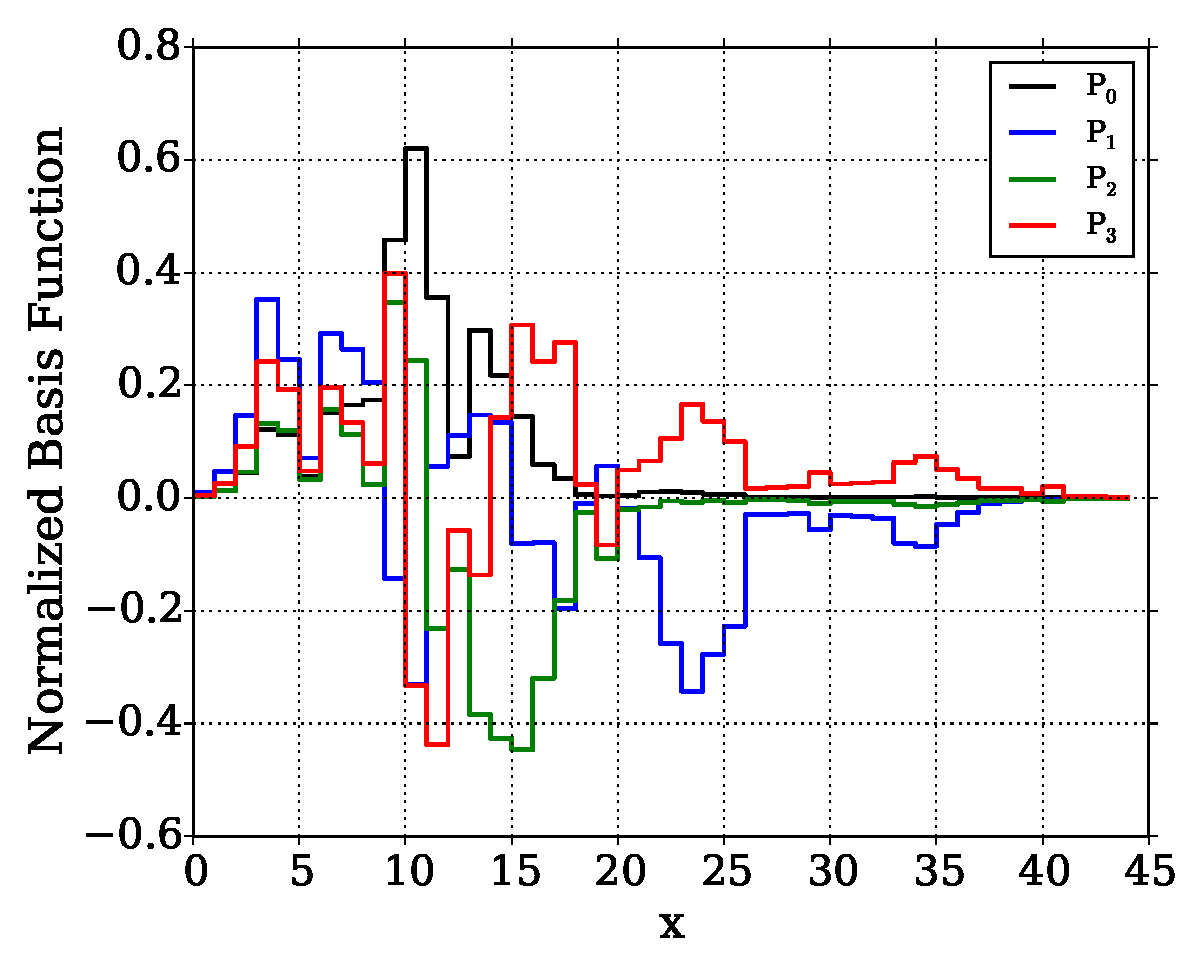
\includegraphics[trim=.1cm .25cm .1cm .4cm, clip=true,
                totalheight=0.65\textheight]{Figures/KLT_basis}
            \end{column}
        \end{columns}
    \end{frame}

    \section{C5G7 Test Problem and Models}

    \begin{frame}
        \frametitle{C5G7 Test Problem}
        \begin{columns}[T]
            \begin{column}{0.5\textwidth}
                \begin{block}{Pin Cell Mesh}
                    \begin{itemize}
                        \item 7$\times$7 Cartesian mesh
                        \item Each pin cell provides 49 energy-dependent
                        snapshots
                    \end{itemize}
                \end{block}
            \end{column}
            \begin{column}{0.5\textwidth}
                \centering
                \begin{figure}
                    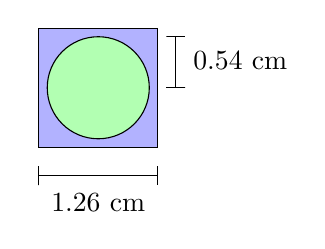
\begin{tikzpicture}[scale=1.2, every node/.style={scale=1}]
                        \filldraw[xshift=0 cm, yshift=0 cm, fill=blue!30!white,
                        draw=black]
                        (0, 0) rectangle (1.26,1.26) node[pos=.5] {};
                        \filldraw[xshift=0 cm, yshift=0 cm, fill=green!30!white,
                        draw=black]
                        (.63,.63) circle (.54) node[pos=.5] {};
                        \draw (0,-.2) -- (0,-.4) -- (0,-.30) -- (0.63,-.3)
                        node[below=0.1cm]
                        {1.26 cm} -- (1.26,-.30) -- (1.26,-.2) -- (1.26, -.4);
                        \draw (1.35,.63) -- (1.55,.63) -- (1.45,.63) --
                        (1.45,.92)
                        node[right=0.1cm] {0.54 cm} -- (1.45,1.17) --
                        (1.35,1.17) -- (1.55,
                        1.17);
                    \end{tikzpicture}
                \end{figure}
            \end{column}
        \end{columns}
        \begin{block}{Test Problem Settings}
            \begin{itemize}
                \item 16-angle, Gauss-Chebyshev quadrature for polar angle
                \item 16-angle, Abu-Shumays Quadruple Range quadrature for
                azimuthal angle
                \item Diamond difference spatial discretization
                \item Scale-generated, 44-group Cross-section Library
            \end{itemize}
        \end{block}

    \end{frame}

    \begin{frame}
        \frametitle{C5G7 Core Configuration}
        \begin{figure}
            \only<1>{
                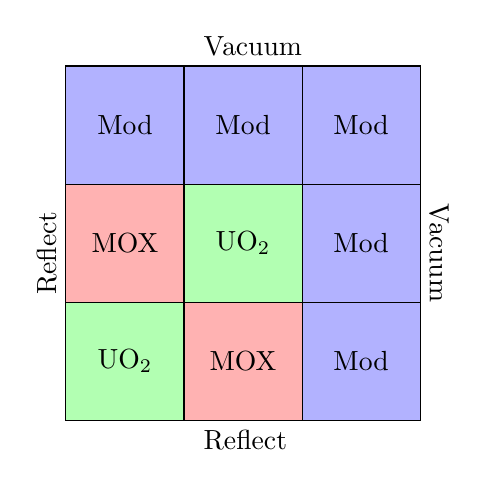
\begin{tikzpicture}[scale=0.5, every node/.style={scale=1}]
                    \filldraw[xshift=6 cm, yshift=0 cm, fill=blue!30!white,
                    draw=black]
                    (0, 0) rectangle (3,3) node[pos=.5] {Mod};
                    \filldraw[xshift=6 cm, yshift=3 cm, fill=blue!30!white,
                    draw=black]
                    (0, 0) rectangle (3,3) node[pos=.5] {Mod};
                    \filldraw[xshift=6 cm, yshift=6 cm, fill=blue!30!white,
                    draw=black]
                    (0, 0) rectangle (3,3) node[pos=.5] {Mod};
                    \filldraw[xshift=3 cm, yshift=6 cm, fill=blue!30!white,
                    draw=black]
                    (0, 0) rectangle (3,3) node[pos=.5] {Mod};
                    \filldraw[xshift=0 cm, yshift=6 cm, fill=blue!30!white,
                    draw=black]
                    (0, 0) rectangle (3,3) node[pos=.5] {Mod};
                    \filldraw[xshift=0 cm, yshift=0 cm, fill=green!30!white,
                    draw=black]
                    (0, 0) rectangle (3,3) node[pos=.5] {UO$_2$};
                    \filldraw[xshift=3 cm, yshift=3 cm, fill=green!30!white,
                    draw=black]
                    (0, 0) rectangle (3,3) node[pos=.5] {UO$_2$};
                    \filldraw[xshift=3 cm, yshift=0 cm, fill=red!30!white,
                    draw=black]
                    (0, 0) rectangle (3,3) node[pos=.5] {MOX};
                    \filldraw[xshift=0 cm, yshift=3 cm, fill=red!30!white,
                    draw=black]
                    (0, 0) rectangle (3,3) node[pos=.5] {MOX};
                    \draw[xshift=9cm,yshift=4.25cm] node[right]
                    {\rotatebox{-90}{Vacuum}};
                    \draw[yshift=4.25cm] node[left] {\rotatebox{90}{Reflect}};
                    \draw[xshift=3.25cm,yshift=9.5cm] node[right] {{Vacuum}};
                    \draw[xshift=3.25cm, yshift=-.5cm] node[right] {{Reflect}};
                \end{tikzpicture}}
            \only<2>{
                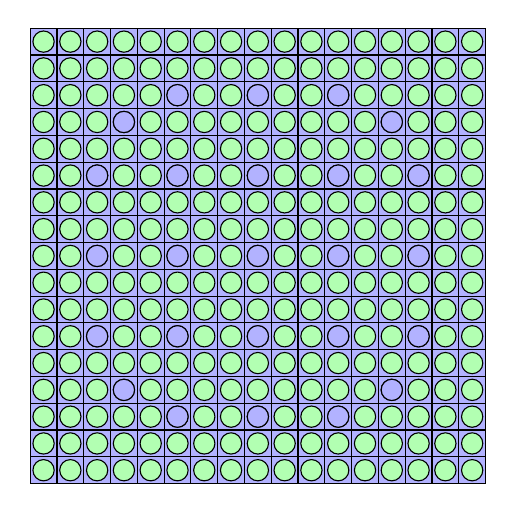
\begin{tikzpicture}[scale=0.27, every node/.style={scale=1}]
                    \foreach \x in {0,1.26,...,20.16}
                    \foreach \y in {0,1.26,...,20.16}
                    \filldraw[xshift=\x cm, yshift=\y cm, fill=blue!30!white,
                    draw=black] (0, 0) rectangle (1.26,1.26) node[pos=.5] {};
                    \foreach \x in {0,1.26,...,20.16}
                    \foreach \y in {0,1.26,...,20.16}
                    \filldraw[xshift=\x cm, yshift=\y cm, fill=green!30!white,
                    draw=black] (.63,.63) circle (.5) node[pos=.5] {};
                    \foreach \x in {5*1.26, 8*1.26, 11*1.26}
                    \foreach \y in {2*1.26, 14*1.26}
                    \filldraw[xshift=\x cm, yshift=\y cm, fill=blue!30!white,
                    draw=black] (.63,.63) circle (.5) node[pos=.5] {};
                    \foreach \x in {3*1.26, 13*1.26}
                    \foreach \y in {3*1.26, 13*1.26}
                    \filldraw[xshift=\x cm, yshift=\y cm, fill=blue!30!white,
                    draw=black] (.63,.63) circle (.5) node[pos=.5] {};
                    \foreach \x in {2*1.26, 5*1.26, 8*1.26, 11*1.26, 14*1.26}
                    \foreach \y in {5*1.26, 8*1.26, 11*1.26}
                    \filldraw[xshift=\x cm, yshift=\y cm, fill=blue!30!white,
                    draw=black] (.63,.63) circle (.5) node[pos=.5] {};
                \end{tikzpicture}}
            \only<3>{
                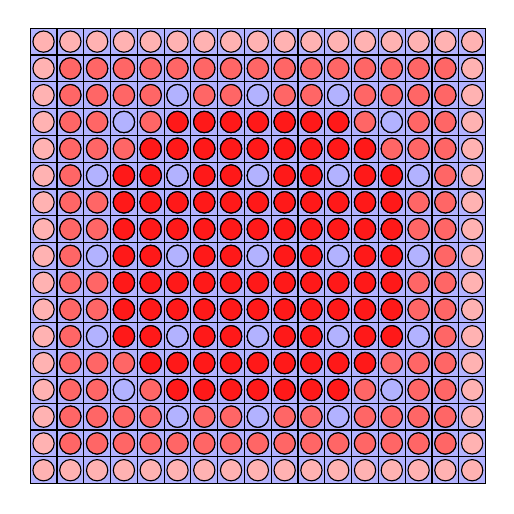
\begin{tikzpicture}[scale=0.27, every node/.style={scale=1}]
                    \foreach \x in {0,1.26,...,20.16}
                    \foreach \y in {0,1.26,...,20.16}
                    \filldraw[xshift=\x cm, yshift=\y cm, fill=blue!30!white,
                    draw=black] (0, 0) rectangle (1.26,1.26) node[pos=.5] {};
                    \foreach \x in {0,1.26,...,20.16}
                    \foreach \y in {0,1.26,...,20.16}
                    \filldraw[xshift=\x cm, yshift=\y cm, fill=red!30!white,
                    draw=black]
                    (.63,.63) circle (.5) node[pos=.5] {};
                    \foreach \x in {1.26,2.52,...,20.16}
                    \foreach \y in {1.26,2.52,...,20.16}
                    \filldraw[xshift=\x cm, yshift=\y cm, fill=red!60!white,
                    draw=black]
                    (.63,.63) circle (.5) node[pos=.5] {};
                    \foreach \x in
                    {5*1.26,6*1.26,7*1.26,8*1.26,9*1.26,10*1.26,11*1.26}
                    \foreach \y in {3*1.26,13*1.26}
                    \filldraw[xshift=\x cm, yshift=\y cm, fill=red!90!white,
                    draw=black]
                    (.63,.63) circle (.5) node[pos=.5] {};
                    \foreach \x in {4*1.26, 5*1.26, 6*1.26, 7*1.26, 8*1.26,
                        9*1.26, 10*1.26, 11*1.26, 12*1.26}
                    \foreach \y in {4*1.26,12*1.26}
                    \filldraw[xshift=\x cm, yshift=\y cm, fill=red!90!white,
                    draw=black]
                    (.63,.63) circle (.5) node[pos=.5] {};
                    \foreach \x in {3.78,5.04,...,16.38}
                    \foreach \y in {6.3,7.56,...,15.04}
                    \filldraw[xshift=\x cm, yshift=\y cm, fill=red!90!white,
                    draw=black]
                    (.63,.63) circle (.5) node[pos=.5] {};
                    \foreach \x in {5*1.26, 8*1.26, 11*1.26}
                    \foreach \y in {2*1.26, 14*1.26}
                    \filldraw[xshift=\x cm, yshift=\y cm, fill=blue!30!white,
                    draw=black] (.63,.63) circle (.5) node[pos=.5] {};
                    \foreach \x in {3*1.26, 13*1.26}
                    \foreach \y in {3*1.26, 13*1.26}
                    \filldraw[xshift=\x cm, yshift=\y cm, fill=blue!30!white,
                    draw=black] (.63,.63) circle (.5) node[pos=.5] {};
                    \foreach \x in {2*1.26, 5*1.26, 8*1.26, 11*1.26, 14*1.26}
                    \foreach \y in {5*1.26, 8*1.26, 11*1.26}
                    \filldraw[xshift=\x cm, yshift=\y cm, fill=blue!30!white,
                    draw=black] (.63,.63) circle (.5) node[pos=.5] {};
                \end{tikzpicture}}
        \end{figure}

        \begin{figure}
            \centering
            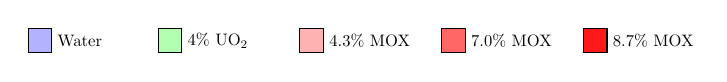
\begin{tikzpicture}[scale=0.6, every node/.style={scale=0.6}]
                \filldraw[xshift=-4cm,fill=blue!30!white,draw=black]
                (-.25,-.25)
                rectangle (.25,.25) node[yshift=-.25cm, right] {Water};%
                \filldraw[xshift=-1.25cm,fill=green!30!white,draw=black](-.25,
                -.25)
                rectangle (.25,.25) node[yshift=-.25cm, right] {4$\%$ UO$_2$};%
                \filldraw[xshift=1.75cm,fill=red!30!white,draw=black]
                (-.25,-.25) rectangle (.25,.25) node[yshift=-.25cm,
                right] {4.3$\%$ MOX};%
                \filldraw[xshift=4.75cm,fill=red!60!white,draw=black]
                (-.25,-.25) rectangle (.25,.25) node[yshift=-.25cm,
                right] {7.0$\%$ MOX};%
                \filldraw[xshift=7.75cm,fill=red!90!white,draw=black]
                (-.25,-.25) rectangle (.25,.25) node[yshift=-.25cm,
                right] {8.7$\%$ MOX};%
            \end{tikzpicture}
        \end{figure}
    \end{frame}

    \begin{frame}
        \frametitle{C5G7 Snapshot Models}
        \begin{table}
            \resizebox{0.9\columnwidth}{!}{%
                \begin{tabular}{l | p{8cm}}\toprule
                    Abbreviation         & Model to generate snapshots \\
                    \midrule
                    Reduced Full-Core    & Spatially averaged snapshots from
                    whole
                    core
                    model (i.e.,         the test problem) \\
                    Combined-Assemblies  & Snapshots from assemblies used in
                    core
                    configuration \\
                    Combined-Pins        & Snapshots from pins used in core
                    configuration combined with the pin
                    junctions\\
                    Small-Core           & Snapshots from the small core model
                    \\
                    Small-Assemblies     & Snapshots from the small assemblies
                    used
                    in the
                    small core configuration \\
                    Reduced Small-Core   & Spatially averaged snapshots from
                    the
                    small core
                    model \\
                    1-D Approximation    & Snapshots from the 1-D approximation
                    to
                    the C5G7
                    benchmark \\
                    \bottomrule
                \end{tabular}}
        \end{table}
    \end{frame}

    \begin{frame}
        \frametitle{Snapshot Model Configurations}
        \only<1>{
            \begin{block}{}
                \centering
                Pincell Junction Configuration
            \end{block}

            \begin{figure}
                \centering
                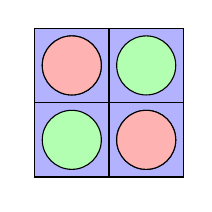
\begin{tikzpicture}[scale=0.75, every node/.style={scale=1}]
                    \foreach \x in {0,1.26}
                    \foreach \y in {0,1.26}
                    \filldraw[xshift=\x cm, yshift=\y cm, fill=blue!30!white,
                    draw=black] (0, 0) rectangle (1.26,1.26) node[pos=.5] {};
                    \foreach \x in {0,1.26}
                    \foreach \y in {0,1.26}
                    \filldraw[xshift=\x cm, yshift=\y cm, fill=green!30!white,
                    draw=black] (.63,.63) circle (.5) node[pos=.5] {};
                    \filldraw[xshift=0 cm, yshift=1.26 cm, fill=red!30!white,
                    draw=black] (.63,.63) circle (.5) node[pos=.5] {};
                    \filldraw[xshift=1.26 cm, yshift=0 cm, fill=red!30!white,
                    draw=black] (.63,.63) circle (.5) node[pos=.5] {};
                \end{tikzpicture}
            \end{figure}}
        \only<2>{
            \begin{block}{}
                \centering
                Small Core Configuration
            \end{block}
            \begin{columns}[T]
                \begin{column}{0.5\textwidth}
                    \begin{figure}
                        \centering
                        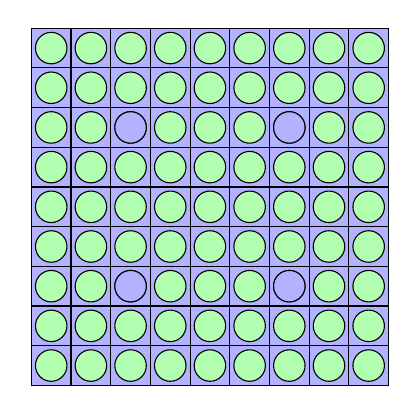
\begin{tikzpicture}[scale=0.4, every
                            node/.style={scale=1}]
                            \foreach \x in {0,1.26,...,10.08}
                            \foreach \y in {0,1.26,...,10.08}
                            \filldraw[xshift=\x cm, yshift=\y cm,
                            fill=blue!30!white,
                            draw=black] (0, 0) rectangle (1.26,1.26)
                            node[pos=.5]
                            {};
                            \foreach \x in {0,1.26,...,10.08}
                            \foreach \y in {0,1.26,...,10.08}
                            \filldraw[xshift=\x cm, yshift=\y cm,
                            fill=green!30!white,
                            draw=black] (.63,.63) circle (.5) node[pos=.5] {};
                            \foreach \x in {2*1.26, 6*1.26}
                            \foreach \y in {2*1.26, 6*1.26}
                            \filldraw[xshift=\x cm, yshift=\y cm,
                            fill=blue!30!white,
                            draw=black] (.63,.63) circle (.5) node[pos=.5] {};
                        \end{tikzpicture}
                    \end{figure}
                \end{column}
                \begin{column}{0.5\textwidth}
                    \begin{figure}
                        \centering
                        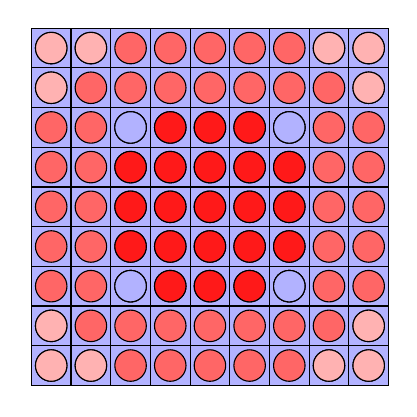
\begin{tikzpicture}[scale=0.4, every
                            node/.style={scale=1}]
                            \foreach \x in {0,1.26,...,10.08}
                            \foreach \y in {0,1.26,...,10.08}
                            \filldraw[xshift=\x cm, yshift=\y cm,
                            fill=blue!30!white,
                            draw=black] (0, 0) rectangle (1.26,1.26)
                            node[pos=.5]
                            {};
                            \foreach \x in {0,1.26,...,10.08}
                            \foreach \y in {0,1.26,...,10.08}
                            \filldraw[xshift=\x cm, yshift=\y cm,
                            fill=red!60!white,
                            draw=black]
                            (.63,.63) circle (.5) node[pos=.5] {};
                            \foreach \x in {0,1.26,7*1.26,10.08}
                            \foreach \y in {0,10.08}
                            \filldraw[xshift=\x cm, yshift=\y cm,
                            fill=red!30!white,
                            draw=black]
                            (.63,.63) circle (.5) node[pos=.5] {};
                            \foreach \x in {0,10.08}
                            \foreach \y in {1.26,7*1.26}
                            \filldraw[xshift=\x cm, yshift=\y cm,
                            fill=red!30!white,
                            draw=black]
                            (.63,.63) circle (.5) node[pos=.5] {};
                            \foreach \x in {2.52,3.78,...,7.56}
                            \foreach \y in {2.52,3.78,...,7.56}
                            \filldraw[xshift=\x cm, yshift=\y cm,
                            fill=red!90!white,
                            draw=black]
                            (.63,.63) circle (.5) node[pos=.5] {};
                            \foreach \x in {2*1.26, 6*1.26}
                            \foreach \y in {2*1.26, 6*1.26}
                            \filldraw[xshift=\x cm, yshift=\y cm,
                            fill=blue!30!white,
                            draw=black] (.63,.63) circle (.5) node[pos=.5] {};
                        \end{tikzpicture}
                    \end{figure}
                \end{column}
            \end{columns}}
        \only<3>{
            \begin{block}{}
                \centering
                1-D Approximation Configuration
            \end{block}
            \begin{figure}
                \centering
                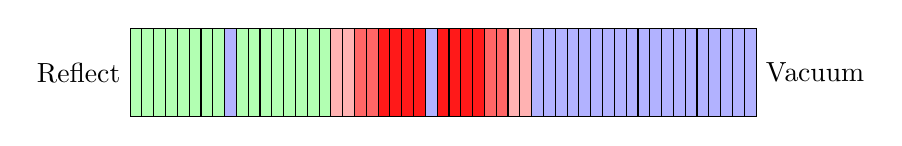
\begin{tikzpicture}[scale=1.5, every node/.style={scale=1}]
                    \foreach \x in {0,.1,...,1.7}
                    \filldraw[xshift=\x cm,fill=green!30!white,draw=black]
                    (0,0)
                    rectangle (0.1,.75);
                    \foreach \x in {1.7,1.8,...,3.4}
                    \filldraw[xshift=\x cm,fill=red!30!white,draw=black] (0,0)
                    rectangle (0.1,.75);
                    \foreach \x in {1.9,2.0,...,3.2}
                    \filldraw[xshift=\x cm,fill=red!60!white,draw=black] (0,0)
                    rectangle (0.1,.75);
                    \foreach \x in {2.1,2.2,...,2.9}
                    \filldraw[xshift=\x cm,fill=red!90!white,draw=black] (0,0)
                    rectangle (0.1,.75);
                    \foreach \x in {3.4,3.5,...,5.3}
                    \filldraw[xshift=\x cm,fill=blue!30!white,draw=black] (0,0)
                    rectangle (0.1,.75);
                    \foreach \x in {0.8,2.5}
                    \filldraw[xshift=\x cm,fill=blue!30!white,draw=black] (0,0)
                    rectangle (0.1,.75);
                    \draw (5.3,.375) node[right] {Vacuum};%
                    \draw (0,.375) node[left] {Reflect};
                \end{tikzpicture}
            \end{figure}
            \begin{figure}
                \centering
                \vspace*{-0.65 cm}
                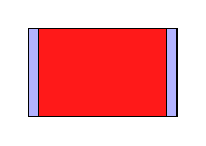
\begin{tikzpicture}[scale=1.5, every node/.style={scale=1}]
                    \filldraw[xshift=0 cm,fill=blue!30!white,draw=black] (0,0)
                    rectangle (.09,.75);
                    \filldraw[xshift=.09 cm,fill=red!90!white,draw=black] (0,0)
                    rectangle (1.17,.75);
                    \filldraw[xshift=1.17 cm,fill=blue!30!white,draw=black]
                    (0,0)
                    rectangle (.09,.75);
                \end{tikzpicture}
            \end{figure}}
        \begin{figure}
            \centering
            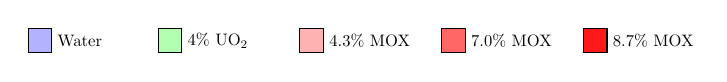
\begin{tikzpicture}[scale=0.6, every node/.style={scale=0.6}]
                \filldraw[xshift=-4cm,fill=blue!30!white,draw=black]
                (-.25,-.25)
                rectangle (.25,.25) node[yshift=-.25cm, right] {Water};%
                \filldraw[xshift=-1.25cm,fill=green!30!white,draw=black]
                (-.25,-.25)
                rectangle (.25,.25) node[yshift=-.25cm, right] {4$\%$ UO$_2$};%
                \filldraw[xshift=1.75cm,fill=red!30!white,draw=black]
                (-.25,-.25) rectangle (.25,.25) node[yshift=-.25cm,
                right] {4.3$\%$ MOX};%
                \filldraw[xshift=4.75cm,fill=red!60!white,draw=black]
                (-.25,-.25) rectangle (.25,.25) node[yshift=-.25cm,
                right] {7.0$\%$ MOX};%
                \filldraw[xshift=7.75cm,fill=red!90!white,draw=black]
                (-.25,-.25) rectangle (.25,.25) node[yshift=-.25cm,
                right] {8.7$\%$ MOX};%
            \end{tikzpicture}
        \end{figure}
    \end{frame}

    \begin{frame}
        \frametitle{Project Goals}
        \begin{block}{Main Objectives}
            \begin{itemize}
                \item Reduce the number of degrees of freedom by an order of
                magnitude
                \item Resolve pin powers or nodal fission densities to
                sub-$0.1\%$ relative errors
            \end{itemize}
        \end{block}
        \begin{block}{Approach}
            \begin{itemize}
                \item Determine a successful basis for energy expansion
                \item Determine constituents of an effective KLT basis
            \end{itemize}
        \end{block}
    \end{frame}

    \section{Results and Analysis}

    \begin{frame}
        \frametitle{C5G7 44-group Library - Nodal Fission Density Results}
        \centering
        Using snapshots of only $\phi$
        \begin{figure}
            \includegraphics[trim=.1cm .25cm 2.0cm .4cm clip=true,
            totalheight=0.75\textheight]{Figures/c/c5g7/rf_plots/phi/%
                energy_basis_comparison_fission-20}
        \end{figure}
    \end{frame}

    \begin{frame}
        \frametitle{C5G7 44-group Library - Nodal Fission Density Results}
        \centering
        Using snapshots of $J_{up}$, and $J_{down}$
        \begin{figure}
            \includegraphics[trim=.1cm .25cm 2.0cm .4cm clip=true,
            totalheight=0.75\textheight]{Figures/s/c5g7/rf_plots/partial/%
                partial_energy_basis_comparison_fission-20}
        \end{figure}
    \end{frame}

    \begin{frame}
        \frametitle{C5G7 44-group Library - Nodal Fission Density Results}
        \centering
        Using snapshots of $\phi$, $J_{up}$, and $J_{down}$
        \begin{figure}
            \includegraphics[trim=.1cm .25cm 2.0cm .4cm clip=true,
            totalheight=0.75\textheight]{Figures/c/c5g7/rf_plots/partial/%
                partial_energy_basis_comparison_fission-20}
        \end{figure}
    \end{frame}

    \begin{frame}
        \frametitle{C5G7 44-group Library - Pin Power Results}
        \centering
        Using snapshots of only $\phi$
        \begin{figure}
            \includegraphics[trim=.1cm .25cm 2.0cm .4cm clip=true,
            totalheight=0.75\textheight]{Figures/c/c5g7/rf_plots/phi/%
                energy_basis_comparison_pinpower-20}
        \end{figure}
    \end{frame}

    \begin{frame}
        \frametitle{C5G7 44-group Library - Pin Power Results}
        \centering
        Using snapshots of $J_{up}$, and $J_{down}$
        \begin{figure}
            \includegraphics[trim=.1cm .25cm 2.0cm .4cm clip=true,
            totalheight=0.75\textheight]{Figures/s/c5g7/rf_plots/partial/%
                partial_energy_basis_comparison_pinpower-20}
        \end{figure}
    \end{frame}

    \begin{frame}
        \frametitle{C5G7 44-group Library - Pin Power Results}
        \centering
        Using snapshots of $\phi$, $J_{up}$, and $J_{down}$
        \begin{figure}
            \includegraphics[trim=.1cm .25cm 2.0cm .4cm clip=true,
            totalheight=0.75\textheight]{Figures/c/c5g7/rf_plots/partial/%
                partial_energy_basis_comparison_pinpower-20}
        \end{figure}
    \end{frame}

    \begin{frame}
        \frametitle{C5G7 44-group Library - Pin Power Heat Map}
        \centering
        Pin power heat map for the {\tt Detran} reference solution.  The
        upper left corner is the center of the core
        \begin{figure}
            \includegraphics[trim=.1cm .25cm 2.0cm .4cm clip=true,
            totalheight=0.75\textheight]{Figures/c/c5g7/rf_plots/%
                c5g7_ref_detran}
        \end{figure}
    \end{frame}

        \begin{frame}
            \frametitle{C5G7 44-group Library - Pin Power Heat Map}
            \centering
            Error in the pin powers of 9th order, Reduced Small-Core, snapshots
            of
            $\phi$ case relative to {\tt Serment}
            reference.
            \begin{columns}[T]
                \begin{column}{0.5\textwidth}
                    \begin{figure}
                        \resizebox{\textwidth}{!}{
                            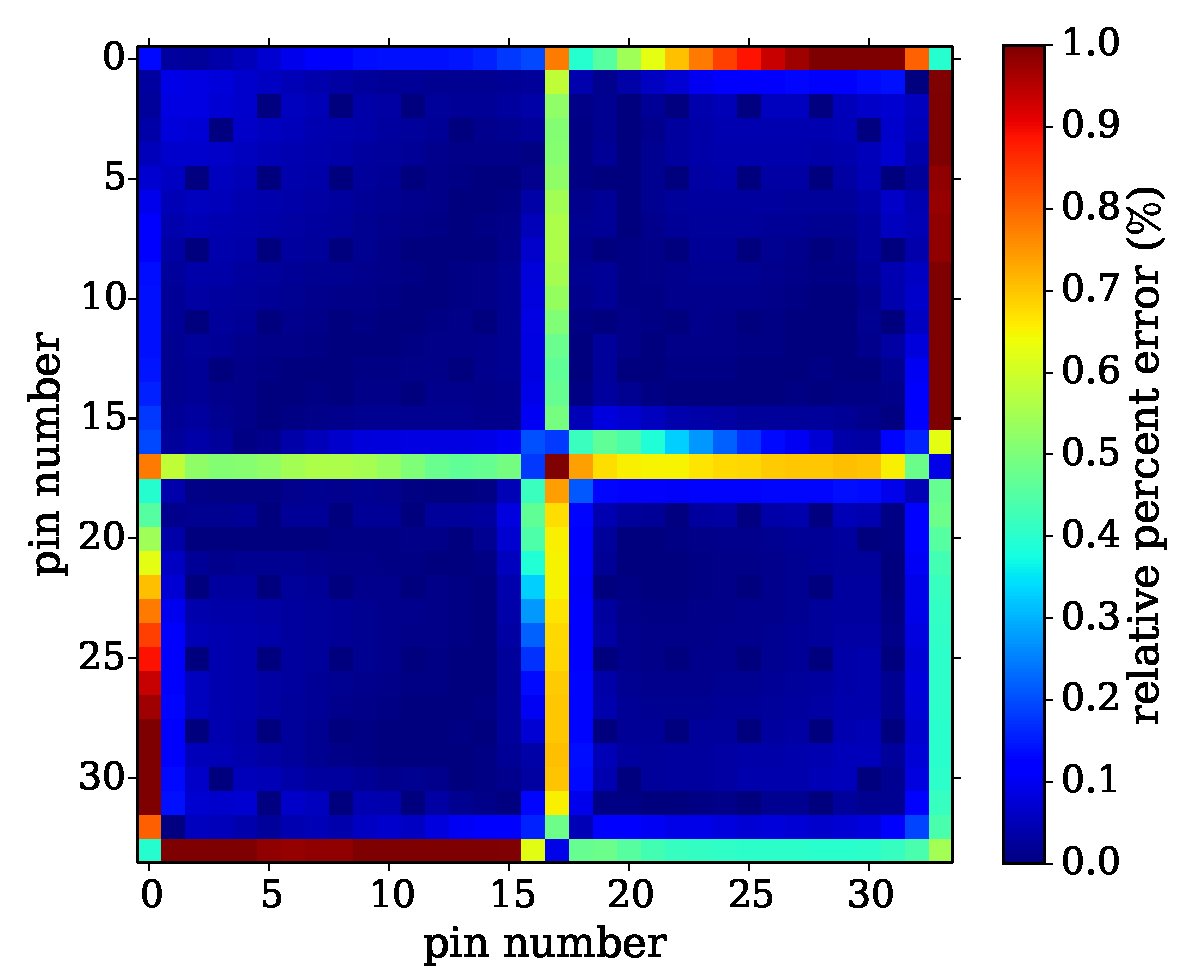
\includegraphics[trim=.1cm .25cm 2.0cm .4cm
                            clip=true,
                            totalheight=0.75\textheight]{%
                                Figures/c/c5g7/rf_plots/phi/serklt8_error}}
                    \end{figure}
                \end{column}
                \begin{column}{0.5\textwidth}
                    \begin{figure}
                        \resizebox{\textwidth}{!}{
                            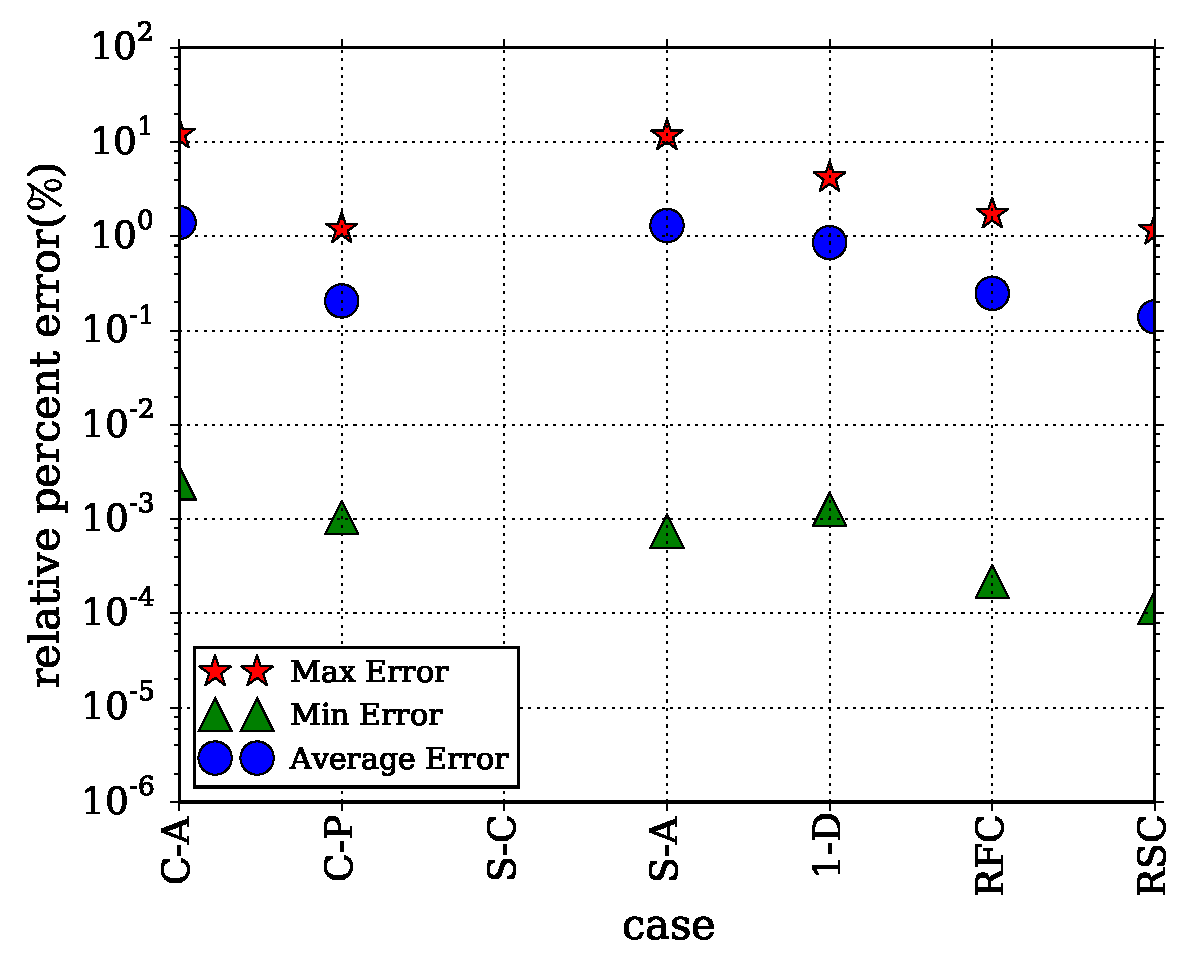
\includegraphics[trim=.1cm .25cm 2.0cm .4cm
                            clip=true,
                            totalheight=0.75\textheight]{%
                                Figures/c/c5g7/rf_plots/error1}}
                    \end{figure}
                \end{column}
            \end{columns}
        \end{frame}

        \begin{frame}
            \frametitle{C5G7 44-group Library - Pin Power Heat Map}
            \centering
            Error in the pin powers of 9th order, Reduced Small-Core, snapshots
            of $J_{up}$, and $J_{down}$ case relative to the
            {\tt Serment} reference solution.
            \begin{columns}[T]
                \begin{column}{0.5\textwidth}
                    \begin{figure}
                        \resizebox{\textwidth}{!}{
                            \includegraphics[trim=.1cm .25cm 2.0cm .4cm
                            clip=true,
                            totalheight=0.75\textheight]{%
Figures/s/c5g7/rf_plots/partial/partial_serklt8_error}}
                    \end{figure}
                \end{column}
                \begin{column}{0.5\textwidth}
                    \begin{figure}
                        \resizebox{\textwidth}{!}{
                            \includegraphics[trim=.1cm .25cm 2.0cm .4cm
                            clip=true,
                            totalheight=0.75\textheight]{%
                                Figures/s/c5g7/rf_plots/partial_error1}}
                    \end{figure}
                \end{column}
            \end{columns}
        \end{frame}

        \begin{frame}
            \frametitle{C5G7 44-group Library - Pin Power Heat Map}
            \centering
            Error in the pin powers of 9th order, Reduced Small-Core, snapshots
            of
            $\phi$, $J_{up}$, and $J_{down}$ case relative to the
            {\tt Serment} reference solution.
            \begin{columns}[T]
                \begin{column}{0.5\textwidth}
                    \begin{figure}
                        \resizebox{\textwidth}{!}{
                            \includegraphics[trim=.1cm .25cm 2.0cm .4cm
                            clip=true,
                            totalheight=0.75\textheight]{%
Figures/c/c5g7/rf_plots/partial/partial_serklt8_error}}
                    \end{figure}
                \end{column}
                \begin{column}{0.5\textwidth}
                    \begin{figure}
                        \resizebox{\textwidth}{!}{
                            \includegraphics[trim=.1cm .25cm 2.0cm .4cm
                            clip=true,
                            totalheight=0.75\textheight]{%
                                Figures/c/c5g7/rf_plots/partial_error1}}
                    \end{figure}
                \end{column}
            \end{columns}
        \end{frame}

        \section{Concluding Remarks}

        \begin{frame}
            \frametitle{Conclusions}
            \begin{block}{Test Problem Conclusions}
                \begin{itemize}
                    \item KLT can make highly successful basis sets
                    \item Material junctions are hardest to capture
                    \item Spatially averaging snapshots provides similar results
                \end{itemize}
            \end{block}
            \begin{block}{The Karhunen Lo\'{e}ve Transform :}
                \begin{itemize}
                    \item Shows improvement over mDLP
                    \item Reduces DOF needed for accurate results
                    \item Generally improves with increased information
                    \item Additional snapshots only improve results if distinct
                    \item Practical snapshot models provide encouraging results
                \end{itemize}
            \end{block}
        \end{frame}

        \begin{frame}
            \frametitle{Future Work}
            \begin{block}{Future Work}
                \begin{itemize}
                    \item Further explore 2-D problems
                    \begin{itemize}
                        \item Higher spatial and angular expansion orders
                    \end{itemize}
                    \item More energy group structures
                    \item Greater snapshot variety (e.g., angular variation)
                    \item Use KLT basis sets to expand {\tt Serment} solution
                    directly
                    \item Application of KLT to additional phase-space
                    expansions
                \end{itemize}
            \end{block}
            \begin{block}{Acknowledgements}
                NRC and the KSU Nuclear Research Fellowship Program
            \end{block}

            \nocite{*}
        \end{frame}

        \begin{frame}[t,allowframebreaks]\label{lastframe}
            \frametitle{References}
            \bibliographystyle{ans}
            {\scriptsize \bibliography{bibliography}}
        \end{frame}

        \beginbackup

        \begin{frame}[noframenumbering]
            \frametitle{Energy Spectra for C5G7 Test Problem}
            \centering
            \begin{figure}
                \begin{columns}[T]
                    \begin{column}{0.5\textwidth}
                        \resizebox{\textwidth}{!}{
                            \includegraphics[trim=.1cm .25cm 2.0cm .4cm
                            clip=true,
                            ]{Figures/c/c5g7/reference_figures/%
                                44group_spectra}}
                    \end{column}
                \end{columns}
            \end{figure}
  \end{frame}

  \backupend

\end{document}
